\chapter{Geografía y teoría económica}

\section{Introdución}

    La agrupación de actividades económicas se puede encontrar en varios niveles de agregación: la variación considerable en el tamaño económico de las ciudades o regiones a nivel nacional, o la distribución desigual de la riqueza y la producción a nivel mundial.\\
    Por supuesto, surge la pregunta de por qué la ubicación parece ser tan importante para las actividades económicas.

\section{La geografía en la economía regional y urbana}
La economía regional y la geografía económica ahora difieren. La economía regional (también conocida como ciencia regional) se basa en la teoría económica neoclásica y es, en efecto, la sucesora formalizada de la tradición alemana de la economía de ubicación. La geografía económica, por otro lado, es más ecléctica y orientada empíricamente. Se inspira en teorías económicas heterodoxas y, cada vez más, en áreas externas a la economía, como la sociología, las ciencias políticas y la teoría de la regulación.\\
Comenzamos con una descripción general de un campo de estudio más joven, a saber, la economía urbana, que estudia la estructura espacial de las áreas urbanas.

\subsection{La economía urbana}
La distribución desigual de la actividad económica dentro de cada país es el punto de partida para la economía urbana. El análisis moderno de la aglomeración de empresas y personas en ciudades o áreas metropolitanas se basa en gran medida en la economía de la aglomeración, un término que se refiere a la disminución de los costos promedio a medida que se produce una mayor producción dentro de un área geográfica específica. En otras palabras se base en rendimientos crecientes a escala. Antes de entrar en la relevancia de las economías de escala para las ciudades y otras formas de aglomeración, primero discutimos un modelo en el que no hay rendimientos crecientes a escala en absoluto. Este modelo, el modelo de ciudad monocéntrica, se origina con von Thu¨nen (1826) y sigue siendo un modelo de referencia para la economía urbana (y regional) hasta el día de hoy. Se justifica una breve discusión, aunque solo sea para poder notar las diferencias con el enfoque de la economía geográfica y dejar claro que, al final, el análisis de las ciudades seguirá siendo bastante limitado mientras no haya rendimientos crecientes a escala.

\subsubsection{El modelo de la ciudad monocéntrica}
El modelo de ciudad monocéntrica asume la existencia de un plano sin rasgos distintivos, perfectamente plano y homogéneo en todos los aspectos. En medio de este plano hay una sola ciudad. Donde existen  agricultores que quieren estar lo más cerca posible de la ciudad para minimizar sus costos de transporte. Este incentivo de estar cerca de la ciudad da como resultado mayores rentas de la tierra cerca de la ciudad que en el borde del plano. Por lo tanto, cada agricultor se enfrenta a una compensación entre las rentas de la tierra y los costos de transporte. Para cada tipo de cultivo existe una curva de oferta-renta que indica, dependiendo de la distancia a la ciudad, cuánto están dispuestos a pagar los agricultores por la tierra.\\
La eficiencia de la asignación de tierras en el modelo monocéntrico depende del supuesto de que no hay externalidades de ubicación.\\
Una serie de hechos estilizados sobre la estructura espacial urbana están de acuerdo con el modelo monocéntrico. Primero, la densidad de población disminuye con la distancia de los centros comerciales centrales. En segundo lugar, casi todas las ciudades importantes del mundo occidental se descentralizaron en el siglo XX (a medida que la gente comenzó a ubicarse más lejos del centro de la ciudad), lo que puede estar relacionado con una caída en los costos de transporte. El modelo monocéntrico también tiene algunas limitaciones serias. Mencionamos solo dos. Primero, el modelo no tiene en cuenta ninguna interacción entre ciudades; no puede ocuparse de los sistemas urbanos. Segundo, el modelo toma la existencia y ubicación de la ciudad como dadas y se enfoca en la ubicación de agricultores/viajeros fuera de la ciudad. \\\\
El término economías de escala o rendimientos crecientes a escala se refiere a una situación en la que un aumento en el nivel de producción implica una disminución en los costos promedio por unidad de producción para la empresa. Se traduce en una curva de costo promedio con pendiente negativa. Para identificar el origen de la caída de los costes medios, Se distingue entre economías de escala internas y externas. Con las economías de escala internas, la disminución de los costes medios se produce por un aumento del nivel de producción de la propia empresa. Cuanto más produce la empresa, mejor puede beneficiarse de las economías de escala y mayor es su ventaja de costos sobre las empresas más pequeñas. La estructura de mercado que subyace a las economías de escala internas, típicamente utilizada en la literatura de economía geográfica, debe ser necesariamente de competencia imperfecta, ya que las economías de escala internas implican poder de mercado.\\
Con las economías de escala externas, la disminución de los costes medios se produce a través de un aumento de la producción a nivel de la industria en su conjunto, lo que hace que los costes medios por unidad sean una función de la producción de toda la industria. Se distingue aquí entre economías externas puras y pecuniarias. Con economías externas puras (o tecnológicas), un aumento en la producción de toda la industria altera la relación tecnológica entre insumos y producción para cada empresa individual. Por lo tanto, tiene un impacto en la función de producción de la empresa. Un ejemplo de uso frecuente (que se remonta a Alfred Marshall; se refiere a los derrames de información (El derrame de conocimiento ocurre cuando las empresas receptoras explotan el conocimiento que ha sido desarrollado originalmente por una empresa de origen). Estas empresas receptoras pueden ser socios de la alianza, competidores directos de la empresa de origen o empresas de otros sectores industriales). Un aumento en la producción de la industria aumenta el acervo de conocimiento a través de los efectos indirectos positivos de información para cada empresa, lo que lleva a un aumento en la producción a nivel de empresa. En la economía urbana, pero también en la nueva teoría del crecimiento y la nueva teoría del comercio se supone que existen economías externas puras. La estructura del mercado puede entonces ser perfectamente competitiva ya que el tamaño de la empresa individual no importa.\\
Las economías externas pecuniarias son transmitidas por el mercado a través de efectos de precio para la empresa individual, lo que puede alterar su decisión de producción. Dos ejemplos, de nuevo basados en Marshall, son la existencia de un gran mercado local de insumos especializados y la puesta en común del mercado laboral. Una gran industria puede respaldar un mercado de insumos intermedios especializados y un grupo de trabajadores calificados específicos de la industria, lo que beneficia a la empresa individual. A diferencia de las economías externas puras, estos efectos indirectos no afectan la relación tecnológica entre insumos y productos (la función de producción). Las externalidades pecuniarias existen en la literatura de economía geográfica a través de un efecto de amor por la variedad en un gran mercado local. La utilidad de cada consumidor depende positivamente del número de variedades que puede comprar de un bien manufacturado. Los efectos de precio cruciales para las externalidades pecuniarias solo pueden ocurrir con competencia imperfecta. Esto es consistente con el requisito de competencia imperfecta para las economías de escala internas, también utilizado en la literatura de economía geográfica. \\
Algunas observaciones finales están en orden. Primero, los derrames o externalidades son cruciales para las economías externas. El concepto de derrames a veces se utiliza solo para economías externas puras, refiriéndose a las economías externas pecuniarias como un caso de interdependencia del mercado. Nos ceñimos al uso de derrames o externalidades cuando nos referimos a economías de escala externas en general. De manera similar, el término "rendimientos crecientes" a veces se usa solo para economías de escala internas. También usamos la frase “rendimientos crecientes” cuando hablamos de economías externas. Del contexto quedará claro si nos referimos al nivel de la empresa o de la industria. En segundo lugar, las economías externas pueden aplicarse a un nivel de agregación superior al de la empresa. Este suele ser el nivel de la industria, pero en la teoría moderna del comercio y la teoría moderna del crecimiento también puede ser la economía en su conjunto. Tercero, las economías externas en los modelos son estáticas, mientras que la literatura también considera economías externas dinámicas. En ese caso, los costos promedio por unidad de producción son una función negativa de la producción acumulada de la industria. Nuevamente, si esto es relevante, quedará claro si nos referimos a economías externas estáticas o dinámicas. Cuarto, las economías externas discutidas anteriormente son positivas pero también pueden ser negativos, es decir, un aumento en la producción de una empresa conduce a un aumento en los costos por unidad para otras empresas. Finalmente, una observación sobre la terminología un tanto confusa con respecto a las externalidades económicas regionales o efectos indirectos. Es habitual distinguir entre las externalidades Marshall-Arrow-Romer (MAR) y las externalidades de Jacobs. En ambos casos, el énfasis está en los efectos indirectos regionales (específicos de la ubicación), es decir, las empresas deben estar ubicadas lo suficientemente cerca unas de otras para beneficiarse de estas externalidades. Las externalidades SAM se centran en los efectos indirectos específicos del sector y también se conocen como economía de localización. Las externalidades de Jacobs se centran en los efectos indirectos específicos de la ciudad que cruzan los límites entre sectores individuales. Estos también se conocen como economía de la urbanización. Dado que la distinción entre las externalidades MAR y Jacobs como tales no es descriptiva (y por lo tanto no informativa) y la distinción de localización/urbanización puede ser confusa (ya que ambas son específicas de la ubicación), tal vez sea mejor hablar de sector específico y de ciudad.

\begin{center}
    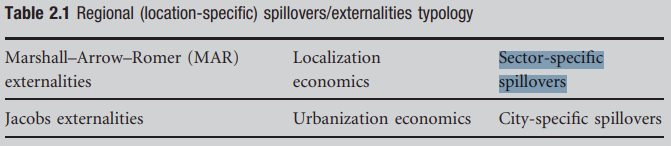
\includegraphics[scale=0.5]{imagen/imagen1.png}
\end{center}

\subsubsection{Economía urbana y rendimientos crecientes}
El punto de partida es bastante diferente del modelo monocéntrico. No hay costes de transporte y el interior de una ciudad ya no forma parte del análisis. En cierto sentido, es un análisis de las ciudades en las que el espacio, es decir, el espacio fuera de las ciudades, no tiene ningún papel que desempeñar. La justificación de este descuido geográfico del espacio no urbano es que, en los países industrializados modernos, una gran parte de la actividad económica general y de la población se encuentra en áreas urbanas, de modo que la relevancia de lo urbano frente a lo no urbano Se supone que las transacciones son limitadas. En cambio, el análisis se centra en las fuerzas que determinan el tamaño de las ciudades y las interacciones entre ellas. La justificación de este descuido geográfico del espacio no urbano es que, en los países industrializados modernos, una gran parte de la actividad económica general y de la población se encuentra en áreas urbanas, de modo que se supone que la relevancia de las transacciones urbanas frente a las no urbanas es limitada. En cambio, el análisis se centra en las fuerzas que determinan el tamaño de las ciudades y las interacciones entre ellas.\\
Las fuerzas de aglomeración en el modelo de Henderson son economías de escala externas positivas que son específicas de la industria. Esto último significa que hay excedentes positivos cuando una empresa de una industria en particular se ubica en una ciudad donde se encuentran otras empresas de la misma industria. \\
Usando una categorización bien conocida que se remonta a los trabajos de Marshall, estos pueden deberse a (i) el intercambio de información, (ii) la existencia de una gran cantidad de mano de obra, o (iii) la existencia de especialistas proveedores. Por lo tanto, las economías externas pueden, en principio, involucrar economías externas puras (como en el enfoque original de Henderson) o economías externas pecuniarias.

\subsubsection{¿Que tipo de economías de escala externas?}
\textbf{Estas economías externas específicas de la industria se conocen como economías de localización, a diferencia de las economías de urbanización.} Si las economías externas son importantes, probablemente sea más importante tener una variedad de industrias diversificadas en una ciudad. Si este último es el caso, surge la pregunta de por qué tantas ciudades están especializadas en industrias particulares. Glaeser et al. (1992: 1148-50) sugieren que tanto las economías de localización como las de urbanización son relevantes (aunque al final favorecen las economías de urbanización), mientras que Duncan Black y Henderson (1999a) argumentan que en un contexto dinámico las economías de localización son más relevantes.\\
Desde un punto de vista teórico, cabe destacar que el enfoque de los sistemas urbanos de Henderson no da por sentada la existencia de la ciudad, como hacía el modelo monocéntrico. También proporciona una teoría de las interacciones entre ciudades. El problema con el enfoque es que el espacio fuera de las ciudades (deliberadamente) no forma parte del análisis. Esto es problemático si uno quiere poder decir dónde están ubicadas las ciudades en relación con otras y la parte no urbana de la geografía: La literatura sobre sistemas de ciudades ha enfatizado el espacio urbano pero ha descuidado el espacio nacional. Como veremos, la ubicación de la actividad manufacturera y la relación entre estas ubicaciones y el resto del espacio es un tema clave en la economía geográfica. Para analizar esta relación, los costos de transporte deben ser parte del análisis, ya que son cruciales para determinar el equilibrio entre las fuerzas de aglomeración y expansión. \\
El uso de rendimientos crecientes y externalidades corresponde a nuestra definición de economías externas puras y economías externas pecuniarias, respectivamente. Ambos tipos de economías externas son importantes. Esto deja la competencia espacial, lo que significa que la competencia entre empresas es casi automáticamente de naturaleza oligopólica cuando se toma en consideración el espacio. La competencia está restringida por la distancia; Por lo general, se piensa que una empresa compite solo con sus empresas vecinas. La competencia espacial está, por tanto, intrínsecamente ligada al comportamiento estratégico de las empresas.  La razón es simplemente que en la economía geográfica y en particular en la versión de competencia monopolística de Avinash Dixit y Joseph Stiglitz (1977) , que caracteriza la estructura del mercado en nuestro modelo central de economía geográfica, el comportamiento estratégico no es tenido en cuenta. Las empresas toman el comportamiento (fijación de precios) de las demás como dado. Además de los tres enfoques mencionados por Fujita y Thisse (1996), Anas, Arnott y Small (1998) dan dos razones adicionales para la aglomeración (urbana): la existencia de un espacio no homogéneo y economías de escala internas en un proceso de producción. Con el primero se puede racionalizar la aglomeración sin ninguna forma de rendimientos crecientes a escala (piense en las diferencias en la geografía física real que da lugar, por ejemplo, a un puerto natural y la aglomeración correspondiente). 

\subsection{Economía regional}
\textbf{La economía regional analiza la organización espacial de los sistemas económicos} (y no solo de las ciudades) y de alguna manera también debe dar cuenta de la distribución desigual en el espacio. von Thu¨nen (1826), Wilhelm Launhardt (1885), Weber (1909), Christaller (1933) y Lo¨sch (1940). Todas estas contribuciones alemanas toman en consideración el espacio nacional o de toda la economía para analizar dónde se ubican las actividades económicas. \\
Esta es una pregunta relevante ya que el movimiento de bienes y personas no es gratuito y la producción suele estar sujeta a alguna forma de rendimientos crecientes. Sin embargo, los padres fundadores de la economía regional se centran en diferentes aspectos de la ubicación de la actividad económica.\\
Von Thu¨nen, por ejemplo, enfatizó las decisiones de ubicación tomadas por los agricultores, mientras que Weber analizó la ubicación óptima y el tamaño de la planta para las empresas manufactureras. Esta sub-sección se centra en las ideas presentadas (y probadas) por primera vez por Christaller y Lo¨sch, \textbf{quienes trataron no solo de explicar la ubicación de las ciudades sino también de diferenciarlas por las diversas funciones que desempeñan y de tratar las relaciones entre las ciudades y el medio ambiente. $"$no ciudades$"$. Este enfoque se conoce como la teoría del lugar central}, que muestra que diferentes puntos o ubicaciones en el panorama económico tienen diferentes niveles de centralidad y que los bienes y servicios se proporcionan de manera eficiente sobre una base jerárquica.

\subsubsection{Teoría del lugar central}
Dada una distribución uniforme de consumidores idénticos en un plano homogéneo, \textbf{la teoría del lugar central sostiene que las ubicaciones difieren en centralidad y que esta centralidad determina el tipo de bienes que proporciona la ubicación.} La provisión de estos bienes está determinada por rendimientos internos crecientes a escala, mientras que la ubicación es relevante porque los consumidores incurren en costos de transporte. Para minimizar estos costos, los consumidores quieren tener acceso a proveedores de bienes cercanos. Para algunos tipos de bienes, como el pan, esto es más fácil que para otros. Por lo tanto, la economía puede sustentar muchos lugares relativamente pequeños (pueblos) donde los panaderos están activos para suministrar pan. Por el contrario, solo puede haber relativamente pocos lugares (ciudades pequeñas, los lugares centrales) donde las empresas de electrónica vendan televisores, que la gente compra con menos frecuencia. Para minimizar los costos de transporte, ambos tipos de ubicaciones se distribuyen de manera bastante uniforme en el espacio. Además, obtenemos una jerarquía de lugares donde la ciudad realiza todas las funciones (vende pan y televisores), mientras que el pueblo realiza solo algunas funciones (vende solo pan). 
El hecho de que se ocupe explícitamente de la ubicación de la actividad económica es una ventaja importante de la teoría del lugar central. El principal problema con el enfoque es que la lógica económica detrás de las decisiones de los consumidores y las empresas sigue sin estar clara. ¿Qué tipo de comportamiento de los agentes individuales conduce a un resultado de lugar central? Los rendimientos crecientes a nivel de empresa requieren alguna forma de competencia imperfecta, un análisis que falta. \\
Los científicos regionales y los geógrafos económicos también han sido conscientes de las limitaciones de esta versión de la teoría del lugar central, que durante los últimos treinta años ha recibido menos interés, particularmente dentro de la geografía económica. Para una base teórica, los geógrafos económicos han comenzado a buscar en otra parte. Sin embargo, siguiendo a Walter Isard (1956, 1960), los científicos regionales han tratado de construir sobre las ideas básicas de la teoría del lugar central para dar una base económica teórica (a menudo altamente formalizada) a esta teoría. Estos modelos son en su mayoría de naturaleza de equilibrio parcial, explicando algunos aspectos del sistema de lugar central mientras ignoran otros. Por lo general, un modelo en esta tradición no trata con empresas o consumidores individuales, sino que formaliza esencialmente el patrón geométrico de un sistema de lugar central. El resultado del lugar central es, por lo tanto, meramente racionalizado y no explicado por el comportamiento subyacente de los consumidores y productores, ni por sus decisiones e interacciones (de mercado). Por ejemplo, la curva de demanda que enfrenta una empresa en un lugar particular no se deriva de los primeros principios, sino que simplemente se supone. 

\subsubsection{Potencial de mercado}
Para el caso de los Estados Unidos, y utilizando el valor de las ventas minoristas por condado de los EE. UU., Harris encuentra que el potencial de mercado de cualquier ubicación se puede describir mediante:
$$MP_i  = \sum_{j=1}^{n}\left(\dfrac{M_j}{D_ij}\right)$$
donde $MP_i$ es el mercado potencial de la ubicación $i$, $M_j$ es la demanda de la ubicación $j$ por los bienes de la ubicación $i$, y $D_{ij}$ es la distancia entre las ubicaciones $i$ y $j$.\\
La idea de que la producción tiene lugar donde la demanda es alta también puede revertirse. La demanda es alta donde se ubica la producción como resultado del poder adquisitivo de los trabajadores que hacen posible la producción en ese lugar.
\subsection{¿Es la economía geográfica nueva? La mirada desde la economía urbana y regional}
Es útil hacer las siguientes dos observaciones sobre el legado de la economía urbana y regional para la economía geográfica y su intento de fundamentar el análisis de la distribución de la actividad económica a través del espacio en un marco de equilibrio general. La primera observación es que el marco estándar de equilibrio general no funcionará si queremos que importen la geografía o el espacio. La existencia de costos positivos de transporte o comercio dará como resultado un equilibrio en el que no habrá transporte ni comercio de bienes.\\
Sin reconocer las indivisibilidades en la persona humana, en las residencias, plantas, equipos y en el transporte los patrones de ubicación, hasta los de la aldea más pequeña, no se pueden entender.\\
Cada ubicación preferirá la autarquía para ahorrar en costos de transporte y, si cada actividad económica es perfectamente (y sin costo) divisible en el espacio, la autarquía o el capitalismo de patio trasero con consumidores/trabajadores autoproductivos es el único resultado factible.\\
Si uno toma los costos de transporte como un hecho inevitable de la vida, debe asumir alguna no homogeneidad del espacio o alguna no convexidad de los conjuntos de producción.\\
La teoría de la ubicación se puede resumir en los siguientes cinco puntos:
\begin{itemize}
    \item El espacio económico es el resultado de una compensación entre varias formas de rendimientos crecientes y diferentes tipos de costos de movilidad,
    \item la competencia de precios, los altos costos de transporte y el uso del suelo fomentan la dispersión de la producción y el consumo; por lo tanto,
    \item es probable que las empresas se concentren en grandes áreas metropolitanas cuando venden productos diferenciados y los costos de transporte son bajos,
    \item las ciudades ofrecen una amplia gama de bienes finales y mercados laborales especializados que las hacen atractivas para los consumidores/trabajadores,
    \item las aglomeraciones son el resultado de procesos acumulativos que involucran tanto a la oferta como a la demanda.
\end{itemize}
\textbf{En consecuencia, la economía espacial debe entenderse como el resultado de la interacción entre las fuerzas de aglomeración y dispersión}.\\
La principal contribución de la economía geográfica es, por lo tanto, combinar los elementos existentes en un solo marco analítico

\section{teoría del comercio internacional}
\textbf{El modelo central de la economía geográfica tiene sus raíces firmemente en la teoría del comercio internacional}

\subsection{Teoría neoclásica del comercio}
La etiqueta teoría neoclásica del comercio se refiere a teorías en las que los flujos comerciales entre naciones se basan en la ventaja comparativa, resultante de las diferencias tecnológicas o de la abundancia de factores. En el modelo de abundancia de factores la ventaja comparativa está determinada, como sugiere el nombre, por las diferencias entre países en la abundancia relativa de las dotaciones de factores. Suponga que hay dos países (Norte y Sur), dos bienes transables (ropa y maquinaria) y dos factores de producción (mano de obra altamente calificada y mano de obra poco calificada). Suponga que el Norte está relativamente bien dotado de mano de obra altamente calificada y el Sur, de mano de obra poco calificada. La producción de ambos conjuntos de bienes requiere ambos insumos, pero la producción de maquinaria es relativamente intensiva en habilidades. Los consumidores del Norte y del Sur tienen preferencias idénticas y consumen ambos bienes. En ausencia de comercio, el Norte, que abunda en mano de obra altamente calificada, puede fabricar maquinaria más fácilmente que el Sur, porque la producción de maquinaria requiere mucha destreza. En la autarquía, esto da como resultado un precio relativamente bajo para la maquinaria en el Norte y la ropa en el Sur. Una vez que el Norte y el Sur comiencen a comerciar, los precios se igualarán, lo que resultará en un precio más alto para la maquinaria en el Norte y un precio más alto para la ropa en el Sur. Como consecuencia, el norte tendrá un incentivo para especializarse (parcialmente) en la producción de maquinaria. Un razonamiento similar es válido para el sur con respecto a la indumentaria. Los flujos comerciales resultantes son del tipo interindustrial (comercio de maquinaria para prendas de vestir). Además, los precios de los factores se igualarán entre el Norte y el Sur como resultado del comercio.
El modelo de abundancia de factores utiliza algunos supuestos específicos adicionales, como competencia perfecta, bienes homogéneos, producción con rendimientos constantes a escala, sin costos de transporte asociados con el comercio de bienes y movilidad de los factores de producción entre industrias, pero no entre países. Está claro que varios de estos supuestos están en desacuerdo con los supuestos clave en la economía regional y urbana, en la que tenemos rendimientos crecientes a escala externos y/o internos, competencia imperfecta, costos de transporte positivos y movilidad de los factores de producción (y las empresas). ¿La geografía o la ubicación de la actividad económica no es un problema en la teoría neoclásica del comercio? Bueno, sí y no. Para explicar esta respuesta, es útil distinguir entre la primera y la segunda naturaleza de la economía de la ubicación. La ubicación de la actividad económica es relevante en el modelo de abundancia de factores en lo que respecta a la distribución desigual de las dotaciones de factores. En nuestro ejemplo, el Norte se especializa en maquinaria y el Sur en ropa como resultado de la distribución geográfica de las dotaciones, lo que se traduce en una distribución desigual de la actividad económica en el espacio global. En este sentido restringido, la geografía importa. \textbf{La ubicación de la producción debería ser una variable endógena, un determinante de ubicación de segunda naturaleza en la terminología de Krugman}. Esta segunda naturaleza está claramente ausente en la teoría de la abundancia de factores. La endogenización de las decisiones de ubicación es necesaria para producir la aglomeración de la actividad económica. Las diferencias en la dotación de factores no pueden implicar un patrón de producción centro-periferia; simplemente conducen a la especialización (en oposición a la aglomeración). El comercio entre países no puede conducir a la desigualdad en el sentido de que la maquinaria y la ropa no pueden aglomerarse en el Norte. El modelo de abundancia de factores conduce a la igualación de los salarios de alta calificación entre el Norte y el Sur (y de manera similar para los salarios de baja calificación).\\
La globalización puede definirse como la creciente interdependencia entre países a través del aumento del comercio y/o el aumento de la movilidad de los factores.\\

Las diferencias relativas en las dotaciones de factores se pueden utilizar para dar una justificación teórica de las diferencias en los patrones de especialización entre países. Otras versiones de la teoría neoclásica del comercio tienen implicaciones similares en lo que se refiere a la relevancia de la geografía. En el modelo ricardiano, la ventaja comparativa, y por lo tanto el patrón comercial, está determinado por las diferencias tecnológicas exógenas entre países. Los países se especializan en la producción de aquellos bienes en los que tienen una productividad comparativamente alta, lo que determina la ubicación de la producción. Nuestra principal objeción al modelo de abundancia de factores también es válida para el modelo ricardiano: en la medida limitada en que la geografía importa, esta relevancia se da de manera exógena. Naturalmente, las diferencias en la dotación de factores o la tecnología pueden ser el resultado de diferencias geográficas. Consideremos, por ejemplo, la tierra como un factor de producción, como en la tradición de von Thunen en economía urbana. La disponibilidad de tierra (fértil) da forma a la ventaja comparativa. De manera similar, la geografía física de un país (acceso al mar, altitud, clima, etc.) también puede ser un determinante subyacente de la ventaja comparativa, que sin duda es válida para el stock de recursos naturales. John Gallup, Jeffrey Sachs y Andrew Mellinger (1998) y Sachs (2003) muestran que tales diferencias geográficas entre países ayudan a explicar las diferencias en el desarrollo económico. Volvemos a este tema en la sección 2.4 y en el capítulo 10, donde discutimos la relevancia de la geografía de primera naturaleza para explicar las diferencias de ingresos entre países cuando se compara con explicaciones contrapuestas.
El papel limitado de la geografía en la teoría neoclásica del comercio quizás se ilustre mejor con el llamado modelo de factores específicos. Parte de la dotación de factores de un país (mano de obra, por ejemplo) es entonces móvil internacionalmente, mientras que otras partes (tierra y capital, por ejemplo) no lo son. La producción de un determinado bien requiere insumos del factor móvil, así como de un factor inmóvil particular o específico (es decir, normalmente tierra o capital específico del sector). Las diferencias en la dotación de los factores específicos influyen así en el patrón de producción y comercio, con un país que se especializa, ceteris paribus, en la producción del bien que requiere el insumo del factor específico con el que el país está relativamente bien dotado. Existe un vínculo geográfico en la medida en que la distribución de las dotaciones inmóviles está determinada por las condiciones geográficas. Una vez más, tal conexión es indirecta en el mejor de los casos, y el impacto de la geografía se determina fuera del modelo comercial.16 Para resumir, Anas, Arnott y Small (1998: 1445) afirman correctamente que el espacio no homogéneo, también conocido como no El espacio neutral, se ha invocado tradicionalmente para explicar la distribución desigual de la actividad económica en la economía internacional. Estos dan lugar a distintas fuentes de ventaja comparativa, que imposibilitan la expansión de la actividad económica. Por lo tanto, la relevancia de la ubicación existe solo por suposición, y no hay interdependencia entre la geografía y la economía. En particular, la ubicación de equilibrio de la actividad económica no es el resultado del comportamiento subyacente de los agentes económicos. El equilibrio (comercial) suele ser único y totalmente determinado por fuerzas exógenas. Más importante aún, la teoría neoclásica del comercio no permite el establecimiento de un equilibrio centro-periferia, lo que presenta un problema en vista de los muchos ejemplos dados en el capítulo 1. Para permitir la aglomeración de la actividad económica, algunos de los supuestos subyacentes a la teoría neoclásica del comercio han Ser cambiado. Un candidato obvio es la introducción de rendimientos internos crecientes a escala y, por lo tanto, de competencia imperfecta (ver subsección 2.3.2). Una observación final sobre la relación entre la geografía y la teoría neoclásica del comercio es que, sin una distribución desigual de los recursos y, por lo tanto, sin una ventaja comparativa, ceteris paribus ya no es una razón fundamental para el comercio, y la geografía deja de ser un problema.17 Introducción positiva costos de transporte, se puede llegar a una conclusión similar incluso si existen ventajas comparativas. Si estos costos son lo suficientemente altos, la producción de bienes estará perfectamente dispersa en el espacio (Ottaviano y Puga, 1997). La economía consistirá entonces en muchas pequeñas empresas, produciendo para su propio consumo: capitalismo de traspatio nuevamente. Esto se relaciona directamente con la discusión del teorema de imposibilidad espacial en la subsección 2.2.3, donde concluimos que una salida era introducir un espacio no homogéneo (la ruta tradicionalmente tomada en la teoría del comercio internacional) y otra salida era introducir un espacio no homogéneo. -convexidades en la producción”, de las cuales los rendimientos crecientes a escala son el mejor ejemplo. A este respecto, la nueva teoría del comercio que se presenta a continuación tiene más en común con la economía urbana y regional que con la teoría neoclásica del comercio.

\subsection{Nueva teoría del comercio}
Se ha desarrollado un modelo en el que los países participan en el comercio que mejora el bienestar incluso cuando no existe ninguna ventaja comparativa. El punto de partida de la nueva teoría del comercio fue el hecho estilizado de que una gran parte del comercio internacional tiene lugar entre países con dotaciones de factores muy similares.\\

\subsubsection{Krugman (1979)}
Las ideas básicas de Krugman (1979) se pueden ilustrar de la siguiente manera. Supongamos que hay dos países con el mismo tamaño de mercado, Oeste y Este, que tienen las mismas dotaciones, usan la misma tecnología y ambos tienen una empresa productora de automóviles. En el modelo de abundancia de factores, estos países no comerciarían. Ambas empresas fabrican varios tipos de automóviles con rendimientos crecientes a escala para cada tipo. En la autarquía, las empresas producen tres tipos de automóviles, a saber, los tipos $X$, $Y$ y $Z$ en el Oeste y los tipos $A$, $B$ y $C$ en el Este. Así, hay una industria que produce seis tipos o variedades de automóviles. Los consumidores (trabajadores) en el Oeste y el Este están inmóviles, distribuidos uniformemente y tienen preferencias idénticas. Las variedades son sustitutos imperfectos y las preferencias son tales que los consumidores siempre prefieren más variedades de un automóvil a menos.  La clave para comprender la justificación del comercio en este modelo es la combinación de rendimientos crecientes a escala a nivel de empresa (economías de escala internas) y el efecto del amor por la variedad en las preferencias de los consumidores, que es una externalidad no tenida en cuenta por las empresas. Al pasar de la autarquía al libre comercio, estos dos supuestos aseguran que el comercio tendrá lugar y mejorará el bienestar. La medida en que cada empresa puede explotar los rendimientos crecientes a escala está determinada por el tamaño del mercado. La apertura del comercio amplía el tamaño del mercado para cada tipo de automóvil. Dado que cada variedad se produce con rendimientos crecientes a escala, este mercado más grande permite a las empresas explotar mejor los rendimientos crecientes. La apertura del comercio significa que la producción de automóviles por variedad puede aumentar a medida que el mercado más grande hace que sea rentable expandir la escala de producción. Al hacerlo, los precios por variedad disminuirán. Para que esto sea posible en el mercado integrado de Occidente y Oriente, el número total de variedades producidas debe disminuir. Para ver esto, tenga en cuenta que las dotaciones totales (Oeste + Este) y el tamaño total del mercado son fijos, de modo que no es posible aumentar simultáneamente la producción de las seis variedades. En libre comercio, los dos países juntos producen menos de seis variedades, digamos cuatro (X, Y, A y B). \textbf{Hay entonces dos efectos positivos sobre el bienestar. Primero, la disminución de los precios provocada por la mayor escala de producción implica que los trabajadores/consumidores terminan con un salario real más alto. En segundo lugar, después del comercio, los consumidores pueden consumir cuatro variedades en lugar de tres, y esto aumenta el bienestar a través del efecto del amor por la variedad.}. La introducción de rendimientos crecientes a escala implica una estructura de mercado de competencia imperfecta. El desafío teórico era, por lo tanto, proporcionar un modelo de comercio con competencia imperfecta. Por suerte, Krugman podía basarse en un modelo de competencia monopolística que acababa de publicarse: Dixit y Stiglitz (1977). El enfoque Dixit-Stiglitz ahora se usa ampliamente en muchos campos, incluida la economía geográfica. Discutimos y explicamos las características principales del modelo Dixit-Stiglitz. En vista de la dificultad de lidiar con la competencia imperfecta, no sorprende que la nueva teoría del comercio también incluya modelos con economías de escala puramente externas, en lugar de internas (Helpman, 1984; Helpman y Krugman, 1985), ya que permite a los economistas geográficos ceñirse a una estructura de mercado de competencia perfecta.  \\
La pregunta ahora es si la nueva teoría del comercio tiene algo que decir sobre el papel de la geografía. En el modelo de Krugman (1979), la respuesta es simple. La ubicación de la actividad económica no es realmente un problema. Los costos comerciales son cero, por lo que las empresas son indiferentes con respecto a la ubicación de sus sitios de producción. Incluso si hay costos comerciales positivos, el tamaño del mercado (exógeno) se distribuye uniformemente entre los dos países, lo que impide cualquier aglomeración de la actividad económica. Es indeterminado qué país termina produciendo qué variedades. Todo lo que se puede decir es que los países producen diferentes variedades y el patrón de comercio es indeterminado. Sin embargo, este modelo es importante como base del modelo central de la economía geográfica, por ejemplo, con respecto al análisis del comportamiento del productor y del consumidor. Con las economías de escala externas tampoco se aborda la ubicación de la actividad económica. Se podría argumentar que los efectos de bloqueo en algunos de estos modelos permiten que las condiciones iniciales desempeñen un papel en la determinación de la asignación de la producción. Al igual que con la teoría del comercio neoclásica, este papel de la geografía se determina fuera del modelo.

\subsubsection{Krugman (1980)}
La justificación del comercio intraindustrial es la misma que en el modelo de 1979, con algunas diferencias notables. En primer lugar, en el modelo de 1980, la apertura del comercio y, por tanto, el aumento del tamaño del mercado, no conduce a un aumento de la escala de producción, a pesar de los rendimientos crecientes a escala a nivel de empresa. En cambio, el volumen de producción de cada variedad (a nivel de empresa) es el mismo bajo la autarquía y el comercio, y los precios no cambian. Las ganancias del comercio ahora se deben completamente al efecto del amor por la variedad, ya que los consumidores pueden elegir entre más variedades bajo comercio que autarquía. En segundo lugar, en el modelo de 1980, el comercio entre naciones incurre en costos de transporte, lo que, obviamente, es relevante desde el punto de vista geográfico. Tercero, en el modelo de 1980, la demanda por variedad ya no es simétrica ya que los países difieren en el tamaño del mercado. Esta distribución desigual del tamaño del mercado se vuelve importante cuando se combina con costos de transporte positivos, porque un país producirá aquellas variedades para las cuales la demanda en el país es relativamente alta. En este sentido, la localización de la producción importa y la concentración de la actividad económica puede ser un resultado del modelo. \textbf{El razonamiento es simple: dada la distribución desigual de la demanda, las empresas, que aún están inmóviles, minimizan los costos de transporte si producen aquellas variedades para las que la demanda interna es relativamente fuerte}. Además, y a diferencia del modelo sin costos de transporte, la dirección del comercio ya no es indeterminada, porque la concentración de la producción implica que los países serán exportadores netos de aquellas variedades para las cuales la demanda interna es relativamente alta. \textbf{Los países tenderán a exportar ese tipo de productos para los que tienen una demanda interna relativamente grande}. Observe que este argumento depende por completo de los rendimientos crecientes; en un mundo de rendimientos decrecientes, \textbf{la fuerte demanda interna de un bien tiende a convertirlo en una importación en lugar de una exportación. Este fenómeno se conoce como el efecto del mercado interno.} Esto sugiere que no hay una diferencia fundamental entre este modelo y el modelo central del capítulo 3. Sin embargo, no estamos de acuerdo con ese punto de vista por tres razones. Primero, ni las empresas ni los trabajadores deciden nada sobre la ubicación en Krugman (1980). No hay movilidad de las empresas ni de los factores de producción. Dada su ubicación (exógena), las empresas toman una decisión solo sobre las variedades que quieren producir. En segundo lugar, la concentración de la producción de variedades (y, por supuesto, de la demanda) no permite la aglomeración de la actividad económica. Los equilibrios centro-periferia no son posibles porque la concentración de la demanda en el primer país, digamos para las variedades X, se refleja en una concentración similar de la demanda para las variedades (1 – X) en el otro país. En este sentido, ambos países se caracterizan por una concentración geográfica de la industria. En tercer lugar, la asignación del tamaño del mercado para las variedades no es un resultado del modelo, sino que simplemente se da (por lo tanto, también se dan los ingresos). Esto está íntimamente ligado a la inmovilidad de los trabajadores (que demandan los bienes producidos) y de las empresas. En estos aspectos, la ubicación en Krugman (1980) todavía se determina fuera del modelo.

\subsubsection{Krugman and Venables (1990)} 
Es un modelo de dos países, en el que el país $1$ es grande: tiene más dotaciones de factores (capital y trabajo) y un mercado más grande que el país 2. En la parte principal de su estudio, las dotaciones relativas son las mismas entre los dos países, por lo que no existe una ventaja comparativa y el comercio es del tipo intraindustrial. Hay dos sectores en ambos países, uno perfectamente competitivo y otro imperfectamente competitivo (manufacturas), ambos productores de bienes transables. El país 1 también tiene un mayor número de empresas en el sector manufacturero. Este sector produce productos diferenciados bajo rendimientos crecientes a escala y competencia monopolística. Se permite la entrada y salida de empresas, pero las empresas no pueden moverse entre países. Esto último también es válido para los factores de producción. Tanto para las empresas como para los factores de producción, sólo existe movilidad intersectorial. La pregunta central es cómo un aumento en el grado de integración económica (utilizando una caída en los costos de transporte como proxy) afecta el centro (país 1) y la periferia (país 2). En la autarquía (cuando los altos costos de transporte prohíben el comercio), ambos países tienen una participación en el sector manufacturero igual a su participación en las dotaciones mundiales. Resulta que, para un rango intermedio de costos de transporte, la integración económica fortalece el centro: la participación del centro en la industria mundial, es mayor que su participación en las dotaciones mundiales, y viceversa para la periferia. Nuevas empresas ingresan al sector manufacturero en el país 1, mientras que algunas empresas salen de este sector en el país 2. Dado el mercado más grande en el país 1 y la minimización de los costos de transporte, las nuevas empresas prefieren el país 1 aunque los salarios sean más altos. A medida que los costos de transporte continúan cayendo, la participación del núcleo de la industria mundial finalmente comienza a disminuir nuevamente. \textbf{A costos de transporte muy bajos, la ventaja de producir en el país con el mercado más grande se vuelve pequeña}, lo que, combinado con la competencia más dura del mercado laboral en el país 1 (más empresas compiten por los factores de producción del país, lo que eleva los precios de los factores), implica que nuevos a las empresas les resulta rentable iniciar la producción en el país 2, donde los salarios son más bajos.  Por lo tanto, no es lineal elación entre la participación de un país en la industria mundial y los costos de transporte.\\
En primer lugar, se ocupa de la aglomeración de la actividad económica, porque permite una distribución global desigual de la actividad manufacturera. En segundo lugar, se basa en ejemplos numéricos y se utilizan para analizar los efectos de la integración económica en el centro y la periferia. Esto se parece a la estrategia de la economía geográfica de utilizar simulaciones por computadora para analizar la aglomeración de la actividad económica. Por lo tanto, surge la pregunta: ¿es este un modelo de economía geográfica completo? La respuesta es que da para mucho, pero al final no lo es. La razón principal es que la existencia de centro y periferia no se deriva del modelo en sí. La suposición de que el los tamaños de mercado difieren plantea la pregunta de por qué debería haber un centro y una periferia para empezar. Además de fijar el tamaño del mercado, se supone que los trabajadores están inmóviles. La movilidad de los trabajadores, y por ende de la demanda, iría en contra de la idea de que se podría fijar a priori el tamaño relativo del mercado de los dos países.\\
El modelo central de los capítulos 3 y 4 agrega la endogenización del tamaño del mercado (y la movilidad de los consumidores/trabajadores, que determinan el tamaño del mercado) al modelo de Krugman y Venables (1990). \\
Se enumeran cuatro características principales de la economía geográfica. Dos de estas características (competencia monopolística Dixit-Stiglitz y costos de transporte tipo iceberg) también están presentes en Krugman (1980). El modelo de Krugman y Venables (1990) agrega un (crudo) intento de usar simulaciones. En nuestra opinión, \textbf{la verdadera novedad de la economía geográfica se encuentra en la cuarta característica, la dinámica, que aborda la cuestión de cómo abordar la movilidad de los agentes económicos (principalmente empresas y trabajadores), que endogeniza el tamaño del mercado.} El énfasis subraya el hecho de que esta es la diferencia clave entre la nueva teoría del comercio y la economía geográfica. Llegamos a la conclusión de que, además de un elemento crucial: la dinámica, los nuevos La teoría del comercio en 1990 era muy similar a la economía geográfica de Krugman (1991a). \\
Desde la perspectiva de la nueva teoría del comercio, Head y Mayer (2004a) lo resumen acertadamente. Enumeran los siguientes cinco ingredientes esenciales de la economía geográfica (2613-4): 
\begin{enumerate}[(i)]
    \item  Rendimientos crecientes a escala que son internos a la empresa;
    \item competencia imperfecta; 
    \item costos positivos de transporte o comercio; 
    \item ubicaciones de empresas endógenas; y 
    \item la ubicación endógena de la demanda, ya sea a través de trabajadores móviles o empresas que utilizan la producción de su sector como insumos intermedios. 
\end{enumerate}
Head y Mayer (2004a: 2614; énfasis en el original) concluyen que los ingredientes [1–4] aparecieron todos en la nueva literatura comercial y, en particular, dieron lugar a los efectos del mercado interno identificados por Krugman (1980). Con estas suposiciones, la aglomeración puede surgir, pero solo a través de la ampliación del tamaño de la región inicial asimetrías. \\
Con los cinco supuestos, se puede romper la simetría inicial y se pueden formar aglomeraciones a través de un proceso de causalidad circular. Cómo la introducción de la condición (5) puede poner en marcha un proceso de causalidad circular; el punto a enfatizar aquí es el importante legado de la nueva teoría del comercio para la economía geográfica. 

\section{Crecimiento económico y desarrollo}
Un descuido geográfico del crecimiento económico no sería un problema en el contexto de nuestro estudio si los países experimentaran un proceso más o menos similar de crecimiento económico y convergieran aproximadamente a los mismos niveles de bienestar económico. Un vistazo rápido a los datos (véanse las figuras 1.2 y 1.3 del capítulo 1) deja claro que no es así. Las tasas de crecimiento del PIB per cápita varían considerablemente entre países, al igual que el nivel del PIB per cápita. Además, los datos sugieren que puede haber un componente geográfico involucrado. Los países de alto y bajo crecimiento suelen estar concentrados geográficamente; piense en el sudeste asiático y el África subsahariana, respectivamente. Los niveles altos y bajos de PIB per cápita claramente tampoco están distribuidos al azar en el espacio: uno observa grupos de países ricos y pobres.

\subsection{Teoría del crecimiento económico}
La geografía no es realmente relevante en la teoría neoclásica del crecimiento. A corto plazo, se puede lograr una tasa de crecimiento positivo de la producción per cápita mediante la acumulación de capital o el progreso tecnológico. Sin embargo, dado que la acumulación de capital está sujeta a la ley de los rendimientos decrecientes (disminución del ingreso marginal de la producción a medida que se añade un factor productivo, manteniendo los otros constantes.), \textbf{solo a través del progreso tecnológico se puede mantener una tasa de crecimiento positivo de la producción per cápita a largo plazo.} El progreso tecnológico es exógeno, de modo que al final deja sin explicación el crecimiento de la producción per cápita. Suponiendo que los países tengan acceso a la misma tecnología y sean iguales en todos los demás aspectos (estructurales o institucionales), la teoría neoclásica del crecimiento predice que los países convergerán al mismo nivel de producción per cápita a largo plazo. El stock de capital (per cápita) será bajo para los países inicialmente pobres, lo que implica un alto retorno de la inversión (acumulación de capital), lo que favorece el proceso de convergencia. Habrá una convergencia absoluta: los países terminarán con el mismo nivel de equilibrio de producción (y capital) per cápita. Aunque la convergencia puede ser lenta, el modelo de crecimiento neoclásico predice que los países pobres se pondrán al día, y que es mejor pensar que las diferencias reales en las tasas de crecimiento reflejan este proceso de convergencia.\\
Bajo la convergencia condicional, los países ya no tienen acceso a la misma tecnología o pueden tener diferentes características institucionales. En consecuencia, no es necesario que los países converjan al mismo nivel de producción per cápita de equilibrio a largo plazo. En cambio, la convergencia está condicionada a las características de un país. Esto permite un vínculo (débil) entre la geografía y la teoría neoclásica del crecimiento: \textbf{en la medida en que las diferencias entre países en tecnología o instituciones sean específicas de la ubicación, la geografía importa.}\\
\textbf{En EEUU se mostró que las diferencias geográficas físicas, como el clima o el acceso al mar, tienen un fuerte impacto en el crecimiento económico.} Al igual que con la teoría neoclásica del comercio, el papel de la geografía en la teoría neoclásica del crecimiento es limitado e indirecto.\\
La nueva teoría del crecimiento, aunque los modelos pueden variar considerablemente, dos diferencias cruciales (entrelazadas) con el modelo de crecimiento neoclásico son los intentos de endogenizar el crecimiento económico y prescindir del supuesto de rendimientos decrecientes de los factores acumulables (van Marrewijk, 1999). Con respecto al uso de economías de escala, existen varias opciones en la nueva literatura sobre crecimiento. Inicialmente, la mayoría de los modelos usaban economías externas puras a nivel nacional o industrial, en lugar de economías internas a nivel de empresa. La investigación posterior también utilizó economías internas positivas bajo competencia imperfecta, similar a la nueva teoría comercial. Las economías externas positivas pueden dar lugar a efectos indirectos positivos y complementariedad estratégica y, por lo tanto, a equilibrios múltiples.\\
También existen otras posibilidades, como el célebre modelo $AK$ con rendimientos constantes del capital a nivel de toda la economía, lo que implica que los países no convergen al mismo equilibrio de largo plazo. La endogenización del proceso de crecimiento se centra en el progreso tecnológico, una función positiva del stock general de capital o mano de obra, o de los gastos en I+D. Sea $Y$ la producción, $K$ el stock de capital, $L$ el trabajo y $A(.)$ la función tecnológica. Considere la siguiente función de producción:

$$Y=A(.)K^{1-b}L^b,\quad 0<b<1$$

Gene Grossman y Helpman (1991) analizan los efectos indirectos localizados si las externalidades positivas asociadas con la I+D o, de manera más general, con el conocimiento existen solo dentro de un determinado grupo de países. Este modelo está muy cerca en varios aspectos del modelo central de la economía geográfica (ver Brakman y Garretsen, 1993: 179). La existencia de externalidades localizadas y, por lo tanto, el rango geográfico limitado de la difusión del conocimiento puede deberse a diferencias culturales, políticas e institucionales, todo lo cual puede contribuir a la localización de estas economías externas. Pueden ayudar a explicar por qué algunos (grupos de) países no solo tienen una tasa de crecimiento y un nivel de producción per cápita más altos que otros, sino también por qué esta diferencia podría no disminuir con el tiempo, haciendo posible el equilibrio centro-periferia.\\
Los nuevos modelos de crecimiento pueden así dar cuenta de la aglomeración de la actividad económica. El problema es cómo se analiza la ubicación en sí. La introducción de la ubicación en la nueva teoría del crecimiento tiene un gran parecido con la relevancia de la ubicación en los modelos de crecimiento neoclásicos que permiten la convergencia condicional. En ambos casos, el papel de la ubicación no se deriva del modelo en sí, y en ambos casos se estipula, ya sea teórica o empíricamente, que la tasa de crecimiento del progreso tecnológico de un país depende de la ubicación de ese país. La conclusión debe ser que la ubicación todavía no forma parte del análisis y que la endogenización del crecimiento económico no se extiende al papel de la geografía. Aunque algunas versiones de la nueva teoría del crecimiento son bastante similares a los modelos de la economía geográfica (rendimientos crecientes a escala, competencia imperfecta, productos diferenciados, equilibrios múltiples), la nueva teoría del crecimiento no ofrece Geografía y teoría económica una teoría de la ubicación.\\\\
Black y Henderson (2003) afirman que el desempeño del crecimiento de \textbf{las ciudades puede diferir por dos razones: diferencias en la geografía física y diferencias debidas a los efectos de concentración enfatizados por la economía geográfica.} Estos últimos los miden a través del mercado potencial de cada ciudad.  \textbf{Con respecto a la geografía física, encuentran que las ciudades en climas cálidos (menos grados día de calentamiento) y más secos (menos precipitaciones) en la costa de hecho crecen más rápido.} En cualquier caso, estos estudios apuntan a la relevancia de la geografía física para explicar la aglomeración de la actividad económica. En un gran estudio entre países, Gallup, Sachs y Mellinger (1998) investigan el impacto de la geografía física en el crecimiento económico. El punto de partida de su análisis es la observación de que prácticamente todos los países de los trópicos son pobres, mientras que los países situados fuera de los trópicos son casi invariablemente relativamente ricos (en PIB per cápita). Además, los países costeros generalmente tienen ingresos más altos que los países sin buen acceso al mar. En una serie de estimaciones transversales, hacen retroceder el crecimiento económico sobre varios indicadores de la geografía física (controlando los determinantes estándar del crecimiento). Ellos también encuentran que la geografía física importa, no necesariamente de manera directa (la ubicación en los trópicos no es significativa pero la presencia de malaria reduce significativamente el crecimiento), pero la importancia de la ubicación de un país frente a la mar (ya sea por ser un país costero o un país con vías navegables que conducen al mar) da un impacto directo directo (positivo) de la geografía física en el crecimiento económico.\\
El punto que queremos enfatizar es que la geografía física es importante para la ubicación de la actividad económica. En la terminología utilizada en este capítulo: los aspectos de primera naturaleza de las elecciones de ubicación son importantes. Es necesario enfatizar esto, porque la economía geográfica,  se enfoca en la segunda naturaleza de la elección de la ubicación, asumiendo a menudo que el espacio (geografía física) es homogéneo. Estos enfoques no están en conflicto entre sí, como también reconocen Gallup, Sachs y Mellinger (1998: 132): Los dos enfoques, por supuesto, pueden ser complementarios: una ciudad puede surgir debido a las ventajas de costos que surgen de la geografía diferenciada, pero continuar prosperar debido a las economías de aglomeración incluso cuando las ventajas de costos han desaparecido.

\subsection{Desarrollo económico}
dentro de la teoría económica, el análisis del desarrollo económico generalmente se refiere a las condiciones bajo las cuales los países en desarrollo pueden lograr el crecimiento económico. Este es un alcance algo más limitado que el análisis del crecimiento económico, que debería aplicarse a todos los países, pero se ocupa más del crecimiento continuo y menos de las condiciones previas para el crecimiento. Hoy en día, los estudios de desarrollo económico hacen un uso extensivo de la teoría del crecimiento económico ya sea antigua y/o nueva). En este sentido, la economía del desarrollo es en gran medida una aplicación de la economía convencional a los países en desarrollo. Pero no siempre fue así ya que este marco fue atacado por su (supuesta) falta de coherencia analítica, lo que no fue del todo sorprendente, porque estos autores, a veces explícitamente pero más a menudo implícitamente, se basó en economías externas y competencia imperfecta, conceptos que no se invocaban con frecuencia en la economía dominante en esos días. \\
Las teorías utilizadas por estos economistas del desarrollo son interesantes no solo porque trataron de explicar las ausentes condiciones para el crecimiento económico en los países en desarrollo, sino porque también tenían un buen ojo para la dimensión geográfica del desarrollo económico, tanto dentro de los países en desarrollo como entre ellos, países ricos y pobres. Esto explica por qué los geógrafos económicos hasta el día de hoy, cuando discuten el desarrollo económico, todavía se refieren al trabajo de estos economistas del desarrollo más antiguos.\\
\textbf{Un tamaño insuficiente del mercado local es visto como la principal causa del subdesarrollo de una región o un país.} La solución al subdesarrollo se encuentra en una expansión coordinada (es decir, dirigida por el gobierno) de la inversión que permita a las empresas cosechar los beneficios de las economías de escala (externas e internas), fomentando así la industrialización de la región o país atrasado. Una empresa individual no tiene incentivos para expandir su nivel de producción debido a la ausencia de rendimientos crecientes a escala a nivel de empresa. La expansión de la producción solo se vuelve rentable, y aquí las economías externas entran en escena, si un número suficiente de otras empresas también expanden su producción, de ahí el término gran impulso.\\
La industrialización en la región o país atrasado también requiere la expansión de la mano de obra manufacturera. Si la mano de obra es inmóvil entre países, la expansión de la mano de obra manufacturera tiene que ocurrir atrayendo mano de obra de otros sectores de la economía (típicamente el sector agrícola), lo que requiere una oferta de mano de obra suficientemente elástica. \\
La existencia de fuertes efectos indirectos localizados conduce al establecimiento de un centro (con un mercado relativamente más grande) y una periferia. Hirschman (1958) también se centra en la naturaleza autorreforzante de diferencias en el desarrollo económico. Su uso de vínculos hacia atrás y hacia adelante puede considerarse como un medio para ilustrar cómo las empresas, al ubicar la producción en una región en particular, aumentan la rentabilidad de otras empresas que lo hacen. En la terminología moderna, las ideas presentadas por Hirschman tienen un claro sabor a rendimientos crecientes a escala. Cabe señalar  que el uso de rendimientos crecientes a escala es (en el mejor de los casos) indirecto, en el sentido de que no analizan del todo la relevancia de las economías de escala para el propio desarrollo económico. Esta relevancia se destila de sus trabajos a través de los ojos de la teoría económica moderna. De hecho, las dificultades para analizar el papel de los rendimientos crecientes y la competencia imperfecta aseguraron que el apogeo de esta rama de la economía del desarrollo fuera bastante efímero. La teoría neoclásica del desarrollo económico, con su énfasis en la competencia perfecta y los rendimientos decrecientes, siguió siendo mucho más influyente. Hoy en día, esta última afirmación ya no se sostiene. Con el surgimiento de la nueva teoría del comercio, la nueva teoría del crecimiento y, por supuesto, la economía geográfica, los rendimientos crecientes y la competencia imperfecta se han convertido más en una regla que en una excepción en la teoría económica. Cuando se trata de desarrollo económico, estas nuevas teorías formalizan las ideas de Rosenstein Rodan cum suis y les dan una base microeconómica.

\section{Conclusión}
Básicamente, todos los enfoques teóricos discutidos en las secciones anteriores tienen algo útil que decir sobre la relación entre geografía y economía, pero que cada enfoque también tiene sus limitaciones. Se puede argumentar que en la economía regional y urbana hay un amplio espacio para la geografía o el espacio en el análisis, pero que estos enfoques a veces carecen de la base microeconómica del comportamiento individual y de la estructura de equilibrio general que constituye la columna vertebral de la corriente principal. Por el contrario, tanto para las viejas como para las nuevas teorías del comercio y el crecimiento, existe tal base microeconómica y una estructura de equilibrio general, pero el problema es que la geografía suele ser casi irrelevante o, cuando importa, su papel no lo es. La economía geográfica puede verse como un intento de romper aún más la valla entre la geografía y la economía. Al hacerlo, tiene sus raíces firmemente en la teoría económica dominante, por lo que es en particular un intento de traer más geografía a la economía. Por esa razón, preferimos el término economía geográfica a nueva geografía económica.\\ 
Finalmente, dado que El estado aislado de von Thunen se publicó en 1826, es bastante desconcertante porqué hasta hace muy poco la corriente principal de la economía descuidó más o menos el tema de la ubicación de la actividad económica. \textbf{Seguramente parte de la respuesta debe ser que el análisis de la ubicación de la actividad económica debe basarse en los rendimientos crecientes a escala y la competencia imperfecta,} y que los economistas han luchado durante mucho tiempo para incorporar ambos estos elementos en sus modelos. De todos modos, esto todavía no puede explicar completamente la negligencia. Tal vez Mark Blaug (1984.

